%\iffalse
\let\negmedspace\undefined
\let\negthickspace\undefined
\documentclass[journal,12pt,onecolumn]{IEEEtran}
\usepackage{cite}
\usepackage{amsmath,amssymb,amsfonts,amsthm}
\usepackage{algorithmic}
\usepackage{graphicx}
\usepackage{textcomp}
\usepackage{xcolor}
\usepackage{txfonts}
\usepackage{listings}
\usepackage{enumitem}
\usepackage{mathtools}
\usepackage{gensymb}
\usepackage{comment}
\usepackage[breaklinks=true]{hyperref}
\usepackage{tkz-euclide} 
\usepackage{listings}
\usepackage{gvv}    
\usepackage{enumitem}
\usepackage{amsmath}
\def\inputGnumericTable{}                                 
\usepackage[latin1]{inputenc}                                
\usepackage{color}                                            
\usepackage{array}                                            
\usepackage{longtable}                                       
\usepackage{calc}                                             
\usepackage{multirow}                                         
\usepackage{hhline}                                           
\usepackage{ifthen}                                           
\usepackage{lscape}
\usepackage{tabularx}
\usetikzlibrary{shapes.gates.logic.US, circuits.logic.US}

\newtheorem{theorem}{Theorem}[section]
\newtheorem{problem}{Problem}
\newtheorem{proposition}{Proposition}[section]
\newtheorem{lemma}{Lemma}[section]
\newtheorem{corollary}[theorem]{Corollary}
\newtheorem{example}{Example}[section]
\newtheorem{definition}[problem]{Definition}
\newcommand{\BEQA}{\begin{eqnarray}}
\newcommand{\EEQA}{\end{eqnarray}}
\newcommand{\define}{\stackrel{\triangle}{=}}
\theoremstyle{remark}
\newtheorem{rem}{Remark}
\begin{document}
\bibliographystyle{IEEEtran}
\vspace{3cm}

\title{GATE:IN-42-2023}
\author{EE23BTECH11025 - Anantha Krishnan $^{}$% <-this % stops a space
}
\maketitle
\bigskip



\section{question}
In the circuit shown, the initial binary content of shift register A is $1101$ and that of shift register B is $1010$. The shift registers are positive-edge triggered, and the gates have no delay.\\
\\
When the shift control is high, what will be the binary content of the shift registers A and B after four clock pulses?\\
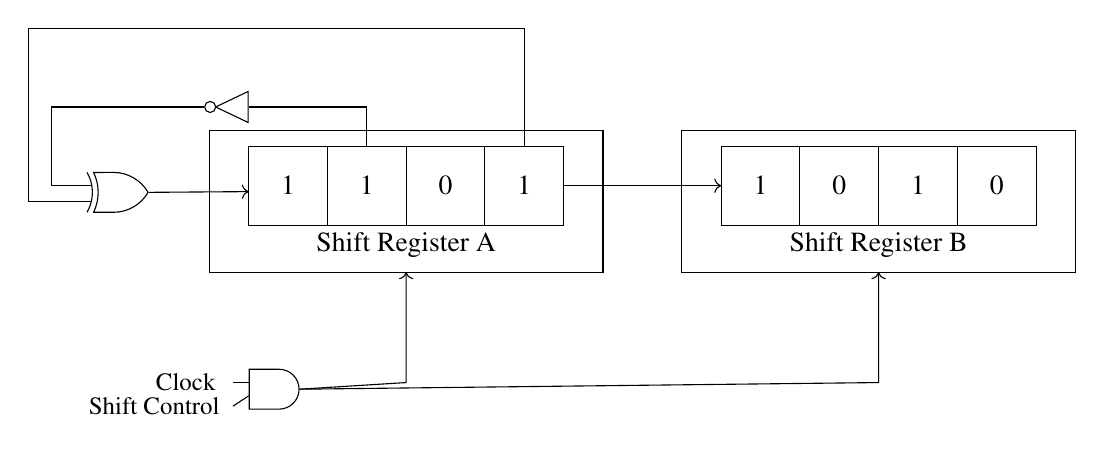
\begin{tikzpicture}

% Outer rectangle for Shift Register A
\draw (-0.5,-0.6) rectangle (4.5,1.2);
\node at (2,-0.25) {Shift Register A};

% Shift Register A
\draw (0,0) rectangle (4,1);
\foreach \i in {1,2,3} {
    \draw (\i,0) -- (\i,1);
}
\node at (0.5,0.5) {1};
\node at (1.5,0.5) {1};
\node at (2.5,0.5) {0};
\node at (3.5,0.5) {1};

% Outer rectangle for Shift Register B
\draw (5.5,-0.6) rectangle (10.5,1.2);
\node at (8,-0.25) {Shift Register B};

% Shift Register B
\draw (6,0) rectangle (10,1);
\foreach \i in {7,8,9} {
    \draw (\i,0) -- (\i,1);
}
\node at (6.5,0.5) {1};
\node at (7.5,0.5) {0};
\node at (8.5,0.5) {1};
\node at (9.5,0.5) {0};

% AND gate for clock and shift control
\node[and gate US, draw, rotate=0, logic gate inputs=nn, anchor=input 1] (andgate) at (0,-2) {};
\node at (-0.8,-2) {\small Clock};
\node at (-1.2,-2.3) {\small Shift Control};

% Connecting lines for AND gate inputs
\draw (-0.2,-2) -- (andgate.input 1);
\draw (-0.2,-2.3) -- (andgate.input 2);

% Arrow from AND gate to Shift Register A
\draw[->] (andgate.output) -- (2,-2) -- (2,-0.6);

% Arrow from AND gate to Shift Register B
\draw[->] (andgate.output) -- (8,-2) -- (8,-0.6);

% Arrow between Shift Register A and B
\draw[->] (4,0.5) -- (6,0.5);

% XOR gate for inputs
\node[xor gate US, draw, anchor=input 1] (xorgate) at (-2,0.5) {};
\draw[->] (xorgate.output) -- (0,0.425);

% Connection from last bit of Shift Register A to XOR gate input
\draw (3.5,1) -- (3.5,2.5) -- (-2.8,2.5) -- (-2.8,0.3) -- (-2,0.3);

% NOT gate and connection from second bit of Shift Register A to XOR gate input
\draw (1.5,1) -- (1.5,1.5) -- (0.5,1.5);
\node[not gate US, draw, rotate= 180, anchor=input] (notgate) at (0,1.5) {};
\draw (notgate.input) -- (0.5,1.5);
\draw (notgate.output) -- (-2.5,1.5) -- (-2.5,0.5) -- (-2,0.5);
\end{tikzpicture}
\begin{enumerate}
    \item  $A = 1101, B=1101$
    \item  $A = 1110, B=1001$
    \item  $A = 0101, B=1101$
    \item  $A = 1010, B=1111$
\end{enumerate}

\end{document}
